\begin{figure*}[p]
    \centering
    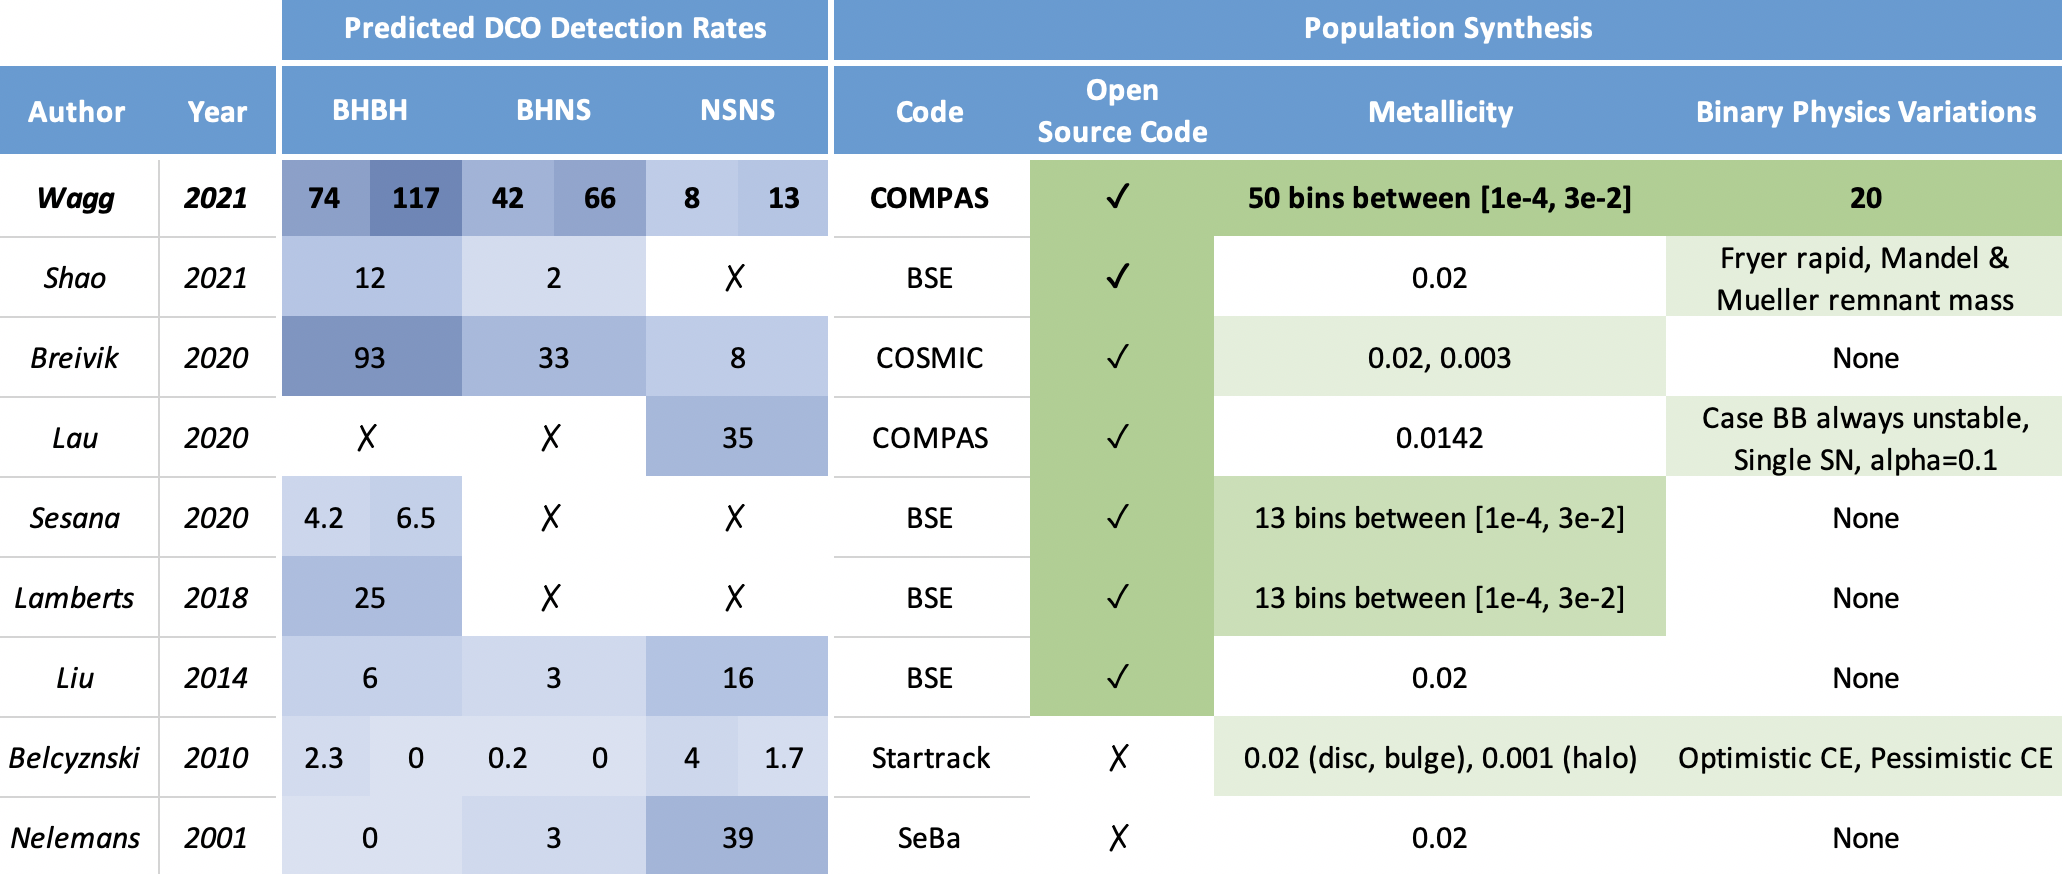
\includegraphics[width=\textwidth]{fig10_1_compare_dco.png}

    \vspace{0.5cm}

    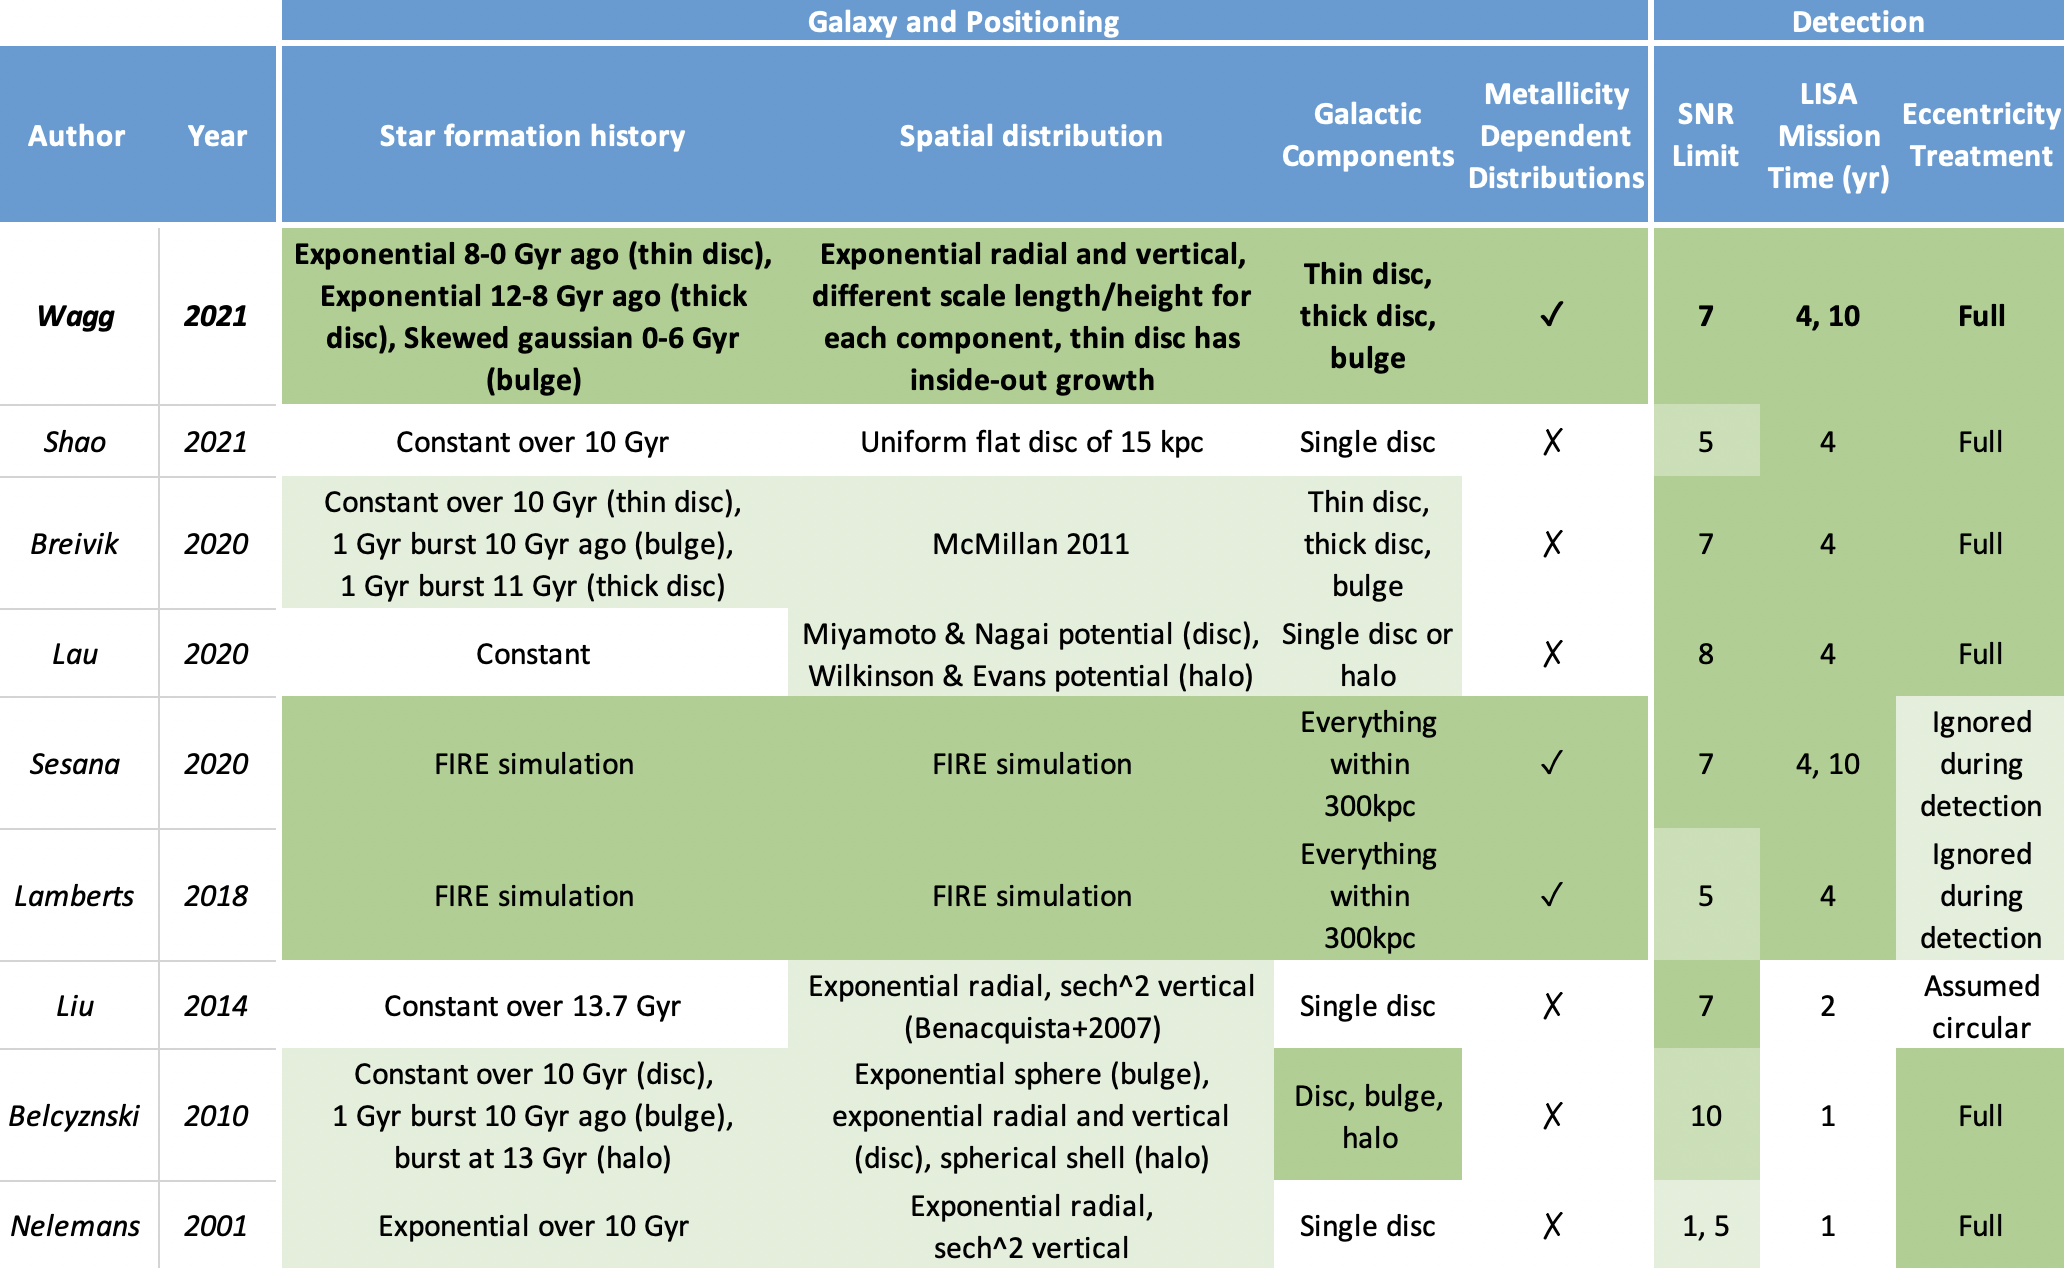
\includegraphics[width=\textwidth]{fig10_2_compare_dco.png}
    \caption{A table comparing previous studies of a similar nature to this work. The works listed in the table are \citet{Nelemans+2001}, \citet{Belczynski+2010}, \citet{Liu+2014}, \citet{Lamberts+2018}, \citet{Sesana+2020}, \citet{Lau+2020}, \citet{Breivik+2020} and \citet{Shao+2021}.}
    \label{fig:previous_studies}
\end{figure*}

In Figure~\ref{fig:previous_studies}, we compare our results to similar previous studies that investigate the population of stellar-mass BHBHs, BHNSs and NSNSs that are detectable with LISA. Figure~\ref{fig:previous_studies} details the expected detection rates predicted by each paper as well as their assumptions regarding their Milky Way galaxy model, binary population synthesis simulation and LISA mission specifications. We only include papers that are similar to our work, such that they use population synthesis and simulate sources in the Galactic plane. Moreover, Figure~\ref{fig:previous_studies} does not include the numerous papers on the LISA WDWD population as we do not make predictions for these DCOs.
 
\paragraph{\citet{Nelemans+2001}} were the first to investigate the population of LISA detectable stellar-mass double compact objects. We find a significantly higher detection rate for BHBHs and BHNSs, as well as a slightly lower rate for NSNSs. We can understand this difference from changes both to the specifications of LISA (such as the mission length and SNR threshold for detection) and our understanding of massive star evolution since the publication of their paper, which both strongly affect the expected detections rates.

\paragraph{\citet{Belczynski+2010}} built upon the work of \citet{Nelemans+2001}, by using a different population synthesis code with two model variations and a multi-component model for the Milky Way. They find a much lower detection rate for BHNSs and NSNSs (and agreed on zero BHBHs) when compared to \citet{Nelemans+2001}. They state that this discrepancy from \citet{Nelemans+2001} comes from differences in their population synthesis and an overall lower formation rate rather than any changes to LISA detectability. The low total detection rate for all DCOs in this paper compared to our work is unsurprising given the relatively high SNR threshold of 10 and short mission length of 1 year. The reduced mission length means that the source signal has much less time to accumulate, whilst also fewer WDWDs can be resolved in this time, leading to a weaker signal and an increased Galactic confusion noise relative to our work.

\paragraph{\citet{Liu+2014}} performed a similar investigation using a different population synthesis code and find higher rates than earlier works. Their lower detection threshold and longer mission length compared to \citet{Belczynski+2010} likely explains the relatively increased rates. Yet their rates are still significantly below what we find. This could be for several reasons; they assume all binaries are circular both in their evolution and for detection. This means that systems may not have inspiralled as far before the LISA mission or may appear to have weaker gravitational waves when eccentricity is not accounted for. They also use a simplified model for the Milky Way with a single disc of one metallicity and constant star formation, whilst also using a mission length half what we assume. Each of these factors likely contributes to the lower overall detection rates.

\paragraph{\citet{Lamberts+2018}} presented a new approach to the problem by using the FIRE simulation \citep{Hopkins+2014} to distribute their sources rather than an analytical model of the Milky Way and were the first paper in this area to incorporate metallicity dependence into their Milky Way model. \citet{Sesana+2020} followed up on this paper using the same simulated BHBH population and presented updated results for the number of expected BHBH detections. They find significantly fewer BHBHs than our fiducial model despite using the same SNR threshold and LISA mission length.
%
The discrepancy between the results of \citet{Sesana+2020} and those presented in this work could be caused by different treatments of eccentricity. Unlike our work, \citet{Sesana+2020} assume that all binaries are circular for the purpose of detection in LISA, which could result in a lower number of detections by missing eccentric binaries that appear as weaker signals when assumed to be circular. This is especially relevant as we find that around $\BHBHNotCirc{}$ of LISA detectable BHBHs are not circular and around $\BHBHHighlyEccentric{}$ have significant eccentricity (see Section~\ref{sec:fiducial_distributions}). We also improve upon this work by using a larger number of metallicity bins compared to \citet{Sesana+2020}, since a low number of metallicity bins can produce artificial features in the mass distribution of DCOs and possibly affect the detection rate (see Appendix~\ref{app:mw_changes}). Finally, it could be that different implicit assumptions in their population synthesis code lead to differences in our results \citep{Toonen+2014}.

\paragraph{\citet{Lau+2020}} focussed on the number of Galactic NSNS binaries that could be detected by LISA. Their study uses the same population synthesis code, COMPAS, as this work, though an earlier version. Despite this, their study finds a much larger number of detections. They make several different physical assumptions in their population synthesis, using the \citet{Fryer+2012} \textit{rapid} remnant mass prescription, limiting the maximum neutron star mass to $2 \unit{M_{\odot}}$ and not implementing PISN. However, we note that none of these assumptions strongly affect the NSNS LISA detection rate (see bottom panel of Fig.~\ref{fig:detection_rates}, models \modRapid{}, \modNSLow{} and \modNoPISN{}) and so this is unlikely to entirely account for our differences. It is also important to highlight that COMPAS has received several improvements and bug fixes since \citet{Vigna-Gomez+2018} (which contains the simulations used by \citet{Lau+2020}) and these could possibly have affected the formation rate of NSNSs.
%
Yet it is most likely that the remaining difference between our results is due to way in which we simulate the Milky Way. \citet{Lau+2020} use a model for the Milky Way similar to that of \citet{Breivik+2020}, which we use to estimate the impact of the choice of MW model is in Appendix~\ref{app:mw_changes}. We find that this simpler model for the Milky Way could result in an overestimation of the NSNS detection rate by at least a factor of two and so this may explain the discrepancy between our results. \citet{Lau+2020} additionally only uses a single metallicity rather than the two used in \citet{Breivik+2020} and so the overestimation could be even stronger as their results will have no contribution from lower metallicity systems.

\paragraph{\citet{Breivik+2020}} introduced the population synthesis code COSMIC and presented detections for many different DCO types in LISA using this code. They find that LISA will detect 93 BHBHs, 33 BHNSs and 8 NSNSs in the Milky Way over a 4 year mission. \citet{Breivik+2020} make many different physical assumptions from us, the most notable being that they assume the optimistic CE scenario and that case BB mass transfer is always unstable, whilst also using a simpler model for the Milky Way (see Appendix~\ref{app:mw_changes}). Thus for better comparison we ran our simulation using model \modCaseBBOpt{} and the Milky Way model from \citet{Breivik+2020}. This results in 97, 101 and 43 detections for BHBHs, BHNSs and NSNSs respectively. Therefore, though we are in very good agreement for BHBHs, we predict much higher rates for BHNSs and NSNSs. These differences are likely due to using a different population synthesis code (COSMIC), which has different underlying physics assumptions from COMPAS. Given our strong agreement for BHBHs, it is possible that COSMIC and COMPAS handle NSs differently and so lead to different detection rates for DCOs containing NSs. However checking this would require a more in-depth study of the intrinsic formation rate of DCOs containing NSs in the two codes.

\paragraph{\citet{Shao+2021}} most recently investigated the detectability binaries containing BHs in LISA using BSE and a relatively simple model for the Milky Way (assuming a uniform flat disc, constant star formation and a single metallicity). They assume that kicks for NSs formed through ECSN are slightly higher than our work ($50 \unit{km}{s^{-1}}$ instead of $30 \unit{km}{s^{-1}}$). This may account for their particularly low BHNS rate (as the binaries would be more likely to disrupt), which is a factor of 20 lower than ours, but we expect their assumption of the optimistic CE scenario, reduced Wolf-Rayet winds and lower SNR detection threshold would offset this. As we show in Appendix~\ref{app:mw_changes}, their use of a simpler Milky Way model, especially with only a single metallicity, would lead to an underestimate of the BHBH and BHNS rates, which may explain the discrepancy in our results.